%\section{Experiments}
%\label{sec:exp}
%In this section, we will introduce our dataset and validate the quality of the dog ``phonemes'', and the dog ``words'' using various methods. We will also outline the experimental details of the sections in the workflow.

%\subsection{Research Questions}
%\XY{TODO}
%RQ2: What is the quality of phone? ()
%RQ3: What is the quality of word? ()
%RQ4: The effect of each step in the workflow? ()


%\subsection{Audio Clean-up}

%\subsection{Dog-Hubert Pretrain}


%\subsection{Evaluation}
%We provide two different evaluations to evaluate the results in two areas, phoneme and lexical. They are complementary and evaluate the phoneme and lexical of dog vocalization understanding.
% \MY{Add a para to say that we provide two different evaluations, which are complementary and evaluating different aspects on dog vocalization understanding.}
% \KZ{Need to get the terminalogy straight in the method section.
% Don't say 5 consecutive labels, u can say phones of at least 5 frames long.
% Define ``frame'' first in the method section.}
\section{Evaluation}
In order to investigate  1) the phones after Dog-HuBert are distinct and accurate 2) the words discovered are complete and semantically-consistent, we evaluate our models' performances on phone recognition accuracy and vocabulary  discovery. 
\subsection{Phone Evaluation}

\paragraph{Setup}

A successfully classified phone should possess the following two properties: 1) same phones should sound very similar; 
and 2) distinct phones should sound different~\citep{freeman1935phoneme}. 
We verify the reliability of phones we got by comparing consecutive identical phone audio samples.
To verify the similarity of phones identified as the same, we randomly sampled 2 audios from different users for
each phone, forming a test set of 140 pairs. To verify the differences between different phones,
we selected the 50 pairs of different phones with the closest cluster centers and randomly sampled 3 audio segments
from different users for each phone, with each segment consisting solely of that phone,
forming a test set of 150 pairs. In total, there are 290 pairs.

The consistency among testers and the result of distinguish identical or distinct phones are indicators for
measuring the reliability of phones.

The testers are two college students majoring in engineering who love small animals and participated in the experiment as volunteers.

%The testers will listen to several pairs of audio segments, including segments with the same label and segments with different labels. The testers are required to use their prior knowledge to judge whether the pair of audio segments belongs to the same category.

\paragraph{Results}

The phone evaluation result is shown in \tabref{tab:phonetestresult}.
Under the condition where the testers' agreement rate is greater than 71\%, 
they can be considered capable of accurately distinguishing same or different phones from an acoustic perspective.

For the internal consistency of each phone, the accuracy of at least 62\% indicates that
the instances from same phone are indeed similar.
Additionally, testers reported that the audio of canine calls was generally similar,
whereas the differences between noises belonging to the same noise label were relatively large.

For the external differences between different phones,
we selected the 50 pairs of phones with the smallest Euclidean distance between their cluster centers, which significantly increased the difficulty of distinguishing these phones. An accuracy rate exceeding 50\% would indicate that these phones are distinct from each other.

\tabref{tab:phonedur} shows the average duration, median duration, and standard deviation of the dog phones and noise labels. The shorter average duration of noise labels and the longer average duration of dog phones further demonstrate the accuracy of phone recognition.

\begin{table}[th]
\centering
\small
\begin{tabular}{lccc}
\hline
\textbf{Tester} & \textbf{AP} & \textbf{SPP} & \textbf{DPP}\\
\hline
\verb|Tester 1| & 58.28\% & 62.86\% & 54.00\%\\
\verb|Tester 2| & 60.00\% & 66.43\% & 54.00\%\\
% \verb|Tester 3| & AudioSep & \pmb{0.7755} \\
\verb|Agreement| & 71.38\% & 75.00\% & 68.00\% \\\hline
\end{tabular}
\caption{Accuracy and agreement result on testing the reliability of phonem discovery. AP: all pairs, SPP: same phone pairs, DPP: different phone pairs.}
\label{tab:phonetestresult}
\end{table}


%During the test, we found that almost $1/3$ of the labels corresponded to noise segments. To this end, two testers conducted a noise-dog sound discrimination experiment on all 50 labels. The experiment randomly selected 5 samples from all 51 labels. The two testers first judged whether the segment was noise from the sound features. If it was impossible to judge from the audio features alone, the testers would refer to the corresponding video for judgment. The judgment results of the two testers are shown in \tabref{tab:phoneclassification}.

%In order to ensure the accuracy of the consistency test of dog sound labels, after excluding noise labels, we finally sampled 30 phoneme labels randomly in dog vocalization labels. Each label has 10 test groups, including five identical label pairs and five different label pairs, for a total of 300 pairs of audio segments. The accuracy is shown in \tabref{tab:phonetestresult}.



%From the test results, we can find that the test results containing only dog sound labels are better than the test data containing noise. At the same time, the testers' judgments on the consistency of the sound are relatively consistent, and the agreement rate is above 80\% on the individual dog labels. According to the feedback from the testers, due to the large number of noise segment types, different types of noise are often classified into the same label within a limited number of labels. The clustering center point results of the audio vector representation of the 50 labels are shown in \figref{fig:cluster}. Due to the model's focus on the context based on transform, noise labels often exist around the dog sound labels, making it difficult for testers to distinguish.

%\MY{Shall we have a comparison with the phoneme labelling results from Jieyi? to show that our method can output better results with higher human agreement}


\begin{table}[th]
\centering
\small
\begin{tabular}{lccc}
\hline
\textbf{} & \textbf{Dog} & \textbf{Noise} & \textbf{All}\\
\hline
\verb|Mean| & 60.51ms & 37.32ms &  52.51ms\\
\verb|Median| & 40ms & 20ms & 40ms\\
\verb|Std| & 65.47ms & 35.29ms & 57.96ms\\\hline
\end{tabular}
\caption{The durations of dog phones and noise labels.}
\label{tab:phonedur}
\end{table}



%Three testers labeled the randomly sampled audio pairs. If the tester considered the audio pair to have the same label, it was marked as 1. If the tester considered the audio pair to have different labels, it was marked as 0. The consistency rate between the model and testers and agreement rate of the three testers' results with the dog vocalization transcription results are shown in \tabref{tab:phonetestresult}.
%\KZ{What do u mean by coincidence? Need to define how you compute these.}\SN{If testers give the ground truth, then we can use accuracy}

%\SN{I will modify this paragraph after get new results}We can see that the coincidence rate of the testers' judgments with the labels we obtained is around 70\%. According to the testers' feedback, about 1/3 of the test samples contained noise, which came from the dog vocalization sentences in the dataset, the judgments result is in Table \ref{tab:phoneclassification}. Due to the wide variety of noise types, several types of noise were classified as the same phoneme by the same label, which made it difficult for the testers to distinguish between noise with the same label and noise with different labels. 
%\KZ{At this point you wanna show a picture of clustering of those noisy labels
%together in the HuBERT embedding space. To back up your claim that those
%are actually noises.} 

%we calculate statistical information for each phoneme,
%as shown in \SN{Table}.
%The average duration of noise phonemes was shorter than canine vocalization phonemes,
%consistent with the characteristics of noise phonemes.

Overall, we have obtained reasonably accurate phone discovery,
both in terms of the internal consistency of instances within the same phone
and the differentiation between phones.
These phones provide a foundation for further exploration into ``words'' in canine language.

\subsection{Lexical Evaluation}

\paragraph{Setup}

To measure the potential semantics within the candidate words we discovery,
we select the 200 of them with the highest occurrence counts in the sentences
after excluding words that contain more than half noise phones.
We also calculated the sentence coverage rate and word length by using the top 100 and top 200 candidate words
to measure the importance of the latter 100 candidate words.

In addition to the properties of the candidate words themselves,
we also calculate the \textbf{reaction CS} score and \textbf{request CS} score for top 200 candidate words in relation to each activity. The higher CS score, the stronger the association between the word and the activity.
Conversely, the closer the CS score is to zero, the weaker the association between the word and the activity.
A negative CS score indicates a negative correlation between the word and the activity.



%\begin{table}
%\centering
%\begin{tabular}{lc}
%\hline
%\textbf{Tester} & \textbf{Accuracy}\\
%\hline
%\verb|Tester 1| & 100 \\
%\verb|Tester 2| & 95 \\
%\verb|Tester 3| & unknown \\ 
%\verb|Agreement| & unknown \\\hline
%\end{tabular}
%\caption{Result of complete word score}
%\label{tab:wordcomplete}
%\end{table}

\paragraph{Results}

%After words discovery step, we have a list of candidate words. T
%
%1. swimming related words.
%
%2. standing and playing with human related words.
%
%3. running related words.
%
%4. standing and taking shower related words.
\begin{figure}[th]
	\centering
	\scalebox{0.45}{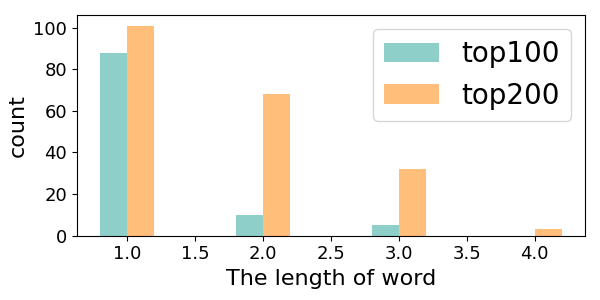
\includegraphics{wordGram.png}}
		\caption{The distribution of word lengths in our dictionary.} 
		\label{fig:wordGram}
\end{figure}
We first look at the top 100 and 200 candidate words obtained by adaptor grammer induction. 
\figref{fig:wordGram} shows the distribution of discovered candidate words over the word length (i.e., unigram, bigram and trigram, etc.). We can see that most candidate
words are shorter but there is a significant amount of bigrams and trigrams in the discovered vocabulary. The average duration of the top 100 candidate words is 0.0637 seconds, while the top 200 candidate words is 0.0719 seconds. The variance duration for the top 100 candidate words is 0.0037 seconds, and for the top 200 candidate words is 0.0047 seconds.

\begin{table}[th]
	\centering
	\small
	\begin{tabular}{lccc}
		\hline
		\textbf{} & \textbf{Sentences~(\%)} & \textbf{Phones~(\%)}\\
		\hline
		top-100 & 89.57 & 80.18 \\
		top-200 & 90.75 & 91.89 \\\hline
	\end{tabular}
	\caption{The coverage of sentences and phones in our vocabulary.}
	\label{tab:wordStats}
\end{table}
Next we look at the coverage of our entire corpus by these top ranked candidate words.
\tabref{tab:wordStats} shows that they cover 90\% of the sentences and also majority
of the phone sequences in the corpus. 

\tabref{tab:actword} shows a set of words that have a causality strength
greater than or equal to 0.07 with each activity. These words are considered
genuine by the framework. Most of these words are bigrams or trigrams. 
One interesting word is 116-46-3, that is a reaction to ``eating'', but it requests
for ``laying down''. After some checking against the raw videos, we realize that 
the eat - bark - laydown procedure happens with a number of dogs, and from the videos, 
we speculate that 116-46-3 is a word that expresses something like ``I'm full''.

\begin{table}[th]
\centering
\small
\begin{tabular}{lcc}
\hline
\textbf{Activity} & \textbf{Word} & \textbf{React/Request}\\
\hline
\verb|Standing| & 59-124-11 & Both \\
\verb|Walking| & 125 & Both\\
\verb|Sitting| & 92-36 & Both \\
\verb|Laying down| & 7-42-22 & React \\
& 116-46-3 & Request \\
\verb|Eating| & 116-46-3 & React\\
& 31-105 & Request \\
\verb|Sleeping| & 126-104 & Both \\
\verb|Running| & 25 & React \\
& 59-74-139 & Request \\
\verb|Taking a shower| & 81-4-81 & Both \\
\verb|Sniffing| & 124-11-104 & Both \\
\verb|Playing(Human)| & 34 & Both \\
\verb|Playing(Toy)| & 38-135 & Both \\
\verb|Swimming| & 113-4-59 & React\\
& 43-25-9 & Request \\
\verb|Begging for food| & 92-36 & React \\
& 128 & Request \\\hline
\end{tabular}
\caption{Activity and their most associated words}
\label{tab:actword}
\end{table}

Then we look the flip side of the experiment and
\tabref{tab:wordact} shows the top activities associated with the top 35 words.
It is interesting to see that there is a strong correlation
between sitting and begging for food, which suggest that
dogs tend to beg for food while sitting, and not standing.
We also find that there are many bigrams, trigrams and even
4-grams in the top 35 words.

\begin{table}[th]
\centering
\small
\begin{tabular}{ll}
\hline
\textbf{Word} & \textbf{Activities} \\
\hline
59-124-11 & standing \\
113-59-124 & standing \\
124-11-104 & standing \\
27-91 & standing, sitting \\
110-31 & standing \\
124-11 & standing, walking \\
59-124-74 & standing \\
11-104 & standing \\
7-42-22 & laying down \\
91-131 & standing \\
59-124 & standing \\
27 & standing \\
46-3 & laying down \\
116-46-3 & laying down \\
128 & sitting, begging for food \\
92-36 & sitting, begging for food \\
7-42-51 & laying down \\
34 & playing with human \\
81-4-81 & sitting, taking shower \\
61-70 & begging for food \\
125 & walking \\
36 & sitting, begging for food \\
5-70 & sitting, begging for food \\
38-135 & laying down \\
113-59-83-17 & laying down \\
59-74-130 & standing \\
57-92 & sitting, begging for food \\
56 & sitting, playing with human \\
51-22 & laying down \\
12-36 & sitting \\
98 & playing with human \\
136 & standing \\
126-4-126 & playing with human \\
66 & standing \\
83-9-16 & begging for food \\\hline
\end{tabular}
\caption{Top 35 words ($CS > 0.07$) and their associated activities}
\label{tab:wordact}
\end{table}


%\begin{table}[th]
%\begin{table}[th]
%	\centering
%	\tiny
%	\begin{tabular}{lccc}
%		\hline
%		\textbf{} & \textbf{Cover sentences~(\%)} & \textbf{Cover phones~(\%)} & \textbf{Word count~(\%)}\\
%		\hline
%		top-100 & 89.57 & 80.18 & 103 \\
%		top-200 & 90.75 & 91.89 & 204 \\\hline
%	\end{tabular}
%	\caption{The Statistical data of words.\XY{where??}}
%	\label{tab:wordStatistic}
%\end{table}

Finally, we assess the accuracy of the top 35 words by human evaluation. Appendix \ref{sec:top}
shows the causal strength of all activities with respective to these words.
We employ three human judges to look at these graphs and label each word as being either
plausible or not plausible based on their reasoning of the relationship between the peak 
activities in each graph. Specifically, if a graph contains a single significant peak, or if
the graph contains multiple peaks, but these peaks have a strong semantic connection, then
the word is considered a plausible word. The annotated results indicate that 87.1\% of the top
35 words are plausible. 
